%%%%%%%%%%%%%%%%%%%%%%%%%%%%%%%%%%%%%%%%%
% Beamer Presentation
% LaTeX Template
% Version 1.0 (10/11/12)
%
% This template has been downloaded from:
% http://www.LaTeXTemplates.com
%
% License:
% CC BY-NC-SA 3.0 (http://creativecommons.org/licenses/by-nc-sa/3.0/)
%
%%%%%%%%%%%%%%%%%%%%%%%%%%%%%%%%%%%%%%%%%

%----------------------------------------------------------------------------------------
%	PACKAGES AND THEMES
%----------------------------------------------------------------------------------------

\documentclass{beamer}
\usefonttheme[onlymath]{serif}

\usepackage{color}
\usepackage{lmodern}
\usepackage{graphicx}

\mode<presentation> {

% The Beamer class comes with a number of default slide themes
% which change the colors and layouts of slides. Below this is a list
% of all the themes, uncomment each in turn to see what they look like.

%\usetheme{default}
%\usetheme{AnnArbor}
%\usetheme{Antibes}
%\usetheme{Bergen}
%\usetheme{Berkeley}
%\usetheme{Berlin}
\usetheme{Boadilla}
%\usetheme{CambridgeUS}
%\usetheme{Copenhagen}
%\usetheme{Darmstadt}
%\usetheme{Dresden}
%\usetheme{Frankfurt}
%\usetheme{Goettingen}
%\usetheme{Hannover}
%\usetheme{Ilmenau}
%\usetheme{JuanLesPins}
%\usetheme{Luebeck}
% \usetheme{Madrid}
%\usetheme{Malmoe}
%\usetheme{Marburg}
%\usetheme{Montpellier}
%\usetheme{PaloAlto}
%\usetheme{Pittsburgh}
%\usetheme{Rochester}
% \usetheme{Singapore}
%\usetheme{Szeged}
%\usetheme{Warsaw}

% As well as themes, the Beamer class has a number of color themes
% for any slide theme. Uncomment each of these in turn to see how it
% changes the colors of your current slide theme.

%\usecolortheme{albatross}
%\usecolortheme{beaver}
%\usecolortheme{beetle}
%\usecolortheme{crane}
%\usecolortheme{dolphin}
%\usecolortheme{dove}
%\usecolortheme{fly}
%\usecolortheme{lily}
%\usecolortheme{orchid}
%\usecolortheme{rose}
%\usecolortheme{seagull}
% \usecolortheme{seahorse}
%\usecolortheme{whale}
%\usecolortheme{wolverine}

%\setbeamertemplate{footline} % To remove the footer line in all slides uncomment this line
%\setbeamertemplate{footline}[page number] % To replace the footer line in all slides with a simple slide count uncomment this line

%\setbeamertemplate{navigation symbols}{} % To remove the navigation symbols from the bottom of all slides uncomment this line
}

\usepackage{graphicx} % Allows including images
\usepackage{booktabs} % Allows the use of \toprule, \midrule and \bottomrule in tables

%----------------------------------------------------------------------------------------
%	TITLE PAGE
%----------------------------------------------------------------------------------------

\title[Image Processing and Chromatic Derivatives]{Image Processing Applications of Chromatic Derivatives} % The short title appears at the bottom of every slide, the full title is only on the title page

\author{Louis Tiao} % Your name
\institute[UNSW] % Your institution as it will appear on the bottom of every slide, may be shorthand to save space
{
School of Computer Science and Engineering, \\
The University of New South Wales \\ % Your institution for the title page
\medskip
\textit{louis.tiao@student.unsw.edu.au} % Your email address
}
\date{\today} % Date, can be changed to a custom date

\begin{document}

\begin{frame}
\titlepage % Print the title page as the first slide
\end{frame}

\begin{frame}
\frametitle{Overview} % Table of contents slide, comment this block out to remove it
\tableofcontents % Throughout your presentation, if you choose to use \section{} and \subsection{} commands, these will automatically be printed on this slide as an overview of your presentation
\end{frame}

%----------------------------------------------------------------------------------------
%	PRESENTATION SLIDES
%----------------------------------------------------------------------------------------

%------------------------------------------------
\section{Introduction} % Sections can be created in order to organize your presentation into discrete blocks, all sections and subsections are automatically printed in the table of contents as an overview of the talk
%------------------------------------------------

\subsection{Motivation} % A subsection can be created just before a set of slides with a common theme to further break down your presentation into chunks

\begin{frame}
\frametitle{Problems in Image Processing}
\framesubtitle{Border handling for kernel convolutions (linear filters)}

Kernel convolution typically requires pixel values from outside the image boundaries.

\begin{columns}[c] % The "c" option specifies centered vertical alignment while the "t" option is used for top vertical alignment
\column{.45\textwidth} % Left column and width
\begin{enumerate}
	\item Extend
	\item Wrap
	\item Crop
	\item \textbf{Approximate} 
\end{enumerate}
\column{.5\textwidth} % Right column and width
\begin{figure} %[!ht]
\centering
	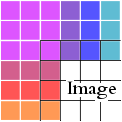
\includegraphics[width=0.3\columnwidth]{../figures/Extend_Edge-Handling}
\caption{Border handling: extend}
\end{figure}
\end{columns}

Make \textbf{local} approximations to extend the image in a visually plausible manner.

\end{frame}

%------------------------------------------------

\begin{frame}
\frametitle{Problems in Image Processing}
\framesubtitle{Digital image inpainting}

Reconstructing lost or deteriorated parts of digital images; removing objects from 
digital images and refilling it in a visually plausible manner.

Existing body of work is dominated by methods involving \textit{texture synthesis} - 
filling holes with repetitive two-dimensional textural patterns. 

\begin{columns}[c] % The "c" option specifies centered vertical alignment while the "t" option is used for top vertical alignment
\column{.45\textwidth} % Left column and width
\begin{enumerate}
	\item Extend \note{nearest border pixels are extended as far as necessary}
	\item Wrap \note{values are taken from opposite corner}
	\item Crop \note{pixels requiring values from beyond the edge are skipped}
	\item \textbf{Approximate} 
\end{enumerate}
\column{.5\textwidth} % Right column and width
\begin{figure} %[!ht]
\caption{Border handling: extend}
\centering
	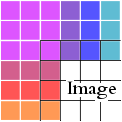
\includegraphics[width=0.3\columnwidth]{../figures/Extend_Edge-Handling}
\end{figure}
\end{columns}

\end{frame}

%------------------------------------------------

\begin{frame}
\frametitle{Image Processing Applications}
\framesubtitle{Digital image inpainting}

Reconstructing lost or deteriorated parts of digital images; removing objects from 
digital images and refilling it in a visually plausible manner.

Existing body of work is dominated by methods involving \textit{texture synthesis} - 
filling holes with repetitive two-dimensional textural patterns. 

\begin{columns}[c] % The "c" option specifies centered vertical alignment while the "t" option is used for top vertical alignment
\column{.45\textwidth} % Left column and width
\begin{enumerate}
	\item Extend \note{nearest border pixels are extended as far as necessary}
	\item Wrap \note{values are taken from opposite corner}
	\item Crop \note{pixels requiring values from beyond the edge are skipped}
	\item \textbf{Approximate} 
\end{enumerate}
\column{.5\textwidth} % Right column and width
\begin{figure} %[!ht]
\caption{Border handling: extend}
\centering
	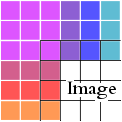
\includegraphics[width=0.3\columnwidth]{../figures/Extend_Edge-Handling}
\end{figure}
\end{columns}
\end{frame}

%------------------------------------------------

\begin{frame}
\frametitle{Fourier series}
\begin{columns}[c]
\column{.6\textwidth}
\begin{itemize}
	\item Let $f(t)$ be a signal in the time domain with period $2T$. Its 
		\textit{Fourier series} expansion is given by

		\begin{align}
			f(t)	&= \sum_{n=-\infty}^{\infty} c_n e^{i \frac{\pi n}{T} t} \\
			c_n		&= \frac{1}{2T} \int_{-T}^{T} f(t) e^{-i \frac{\pi n}{T} t} dt
		\end{align}
	\item \textbf{Global}, approximates local behaviour poorly
	\item Indispensable to digital signal processing (DSP)
	% TODO: Insert complex exponential identities (?)
\end{itemize}
\column{.4\textwidth}
\begin{figure} %[!ht]
\centering
	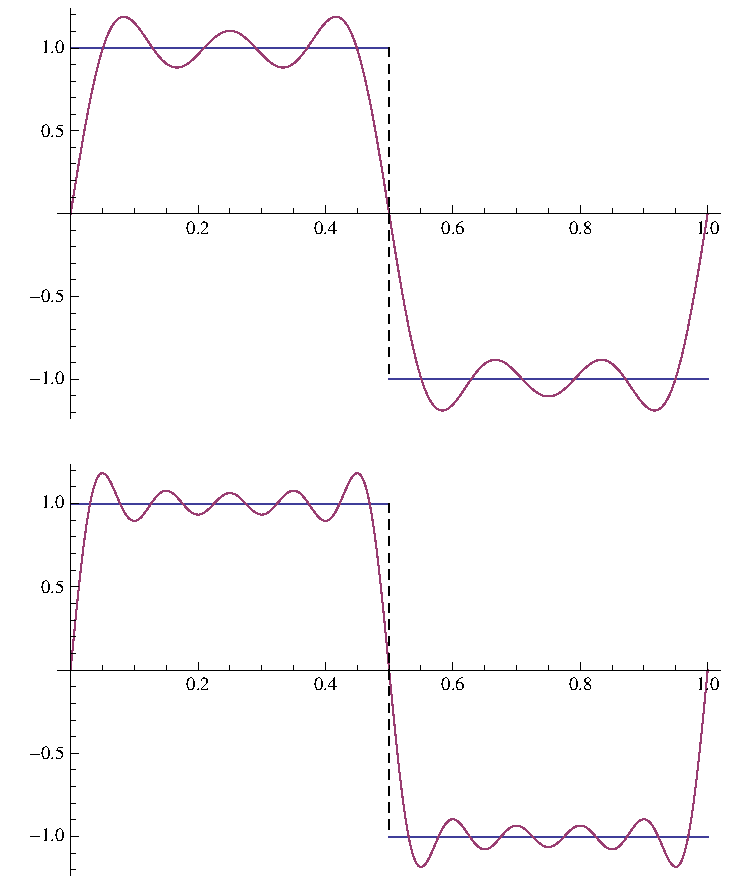
\includegraphics[width=\columnwidth]{../figures/fourier}
\caption{Truncated Fourier expansion with 11 terms (top) and 21 terms (bottom)}
\end{figure}
\end{columns}
\end{frame}

%------------------------------------------------

\begin{frame}
\frametitle{Whittaker-Shannon interpolation formula}
\begin{itemize}
	\item If $f \in \mathbf{BL}(\pi)$, i.e. $f \in L^2$ and $\hat{f}(\omega)$ 
		supported on $[-\pi, \pi]$, we can derive the \textit{Whittaker-Shannon
		interpolation formula}
		\begin{align}
		f(t)	&= \sum_{n=-\infty}^{\infty} f(n) \mathrm{sinc}{\pi(t-n)} \left (
				= \sum_{n=-\infty}^{\infty} f(n) \frac{\sin{\pi(t-n)}}{\pi(t-n)}
				\right )
		\end{align}
	\item \textbf{Global}, approximates local behaviour poorly
	\item Indispensable to digital signal processing (DSP)
\end{itemize}
\end{frame}

%------------------------------------------------

\begin{frame}
\frametitle{Taylor series}
\begin{columns}[c]
\column{.6\textwidth}
\begin{itemize}
	\item The \textit{Taylor series} expansion of $f(t)$ (about point $t=t_0$) is given by

	\begin{align*}
		f(t)	&= \sum_{n=0}^{\infty} c_n \frac{(t-t_0)^n}{n!} \\
		c_n		&= \mathcal{D}^n[f](t_0) = \mathcal{D}_t^n f(t) |_{t=t_0} \\
				&= \frac{d^n}{dt^n} f(t) |_{t=t_0} = f^{(n)}(t_0)
	\end{align*}
	\item \textbf{Local}
	\item Of limited use to DSP. \alert{Why?}
\end{itemize}
\column{.4\textwidth}
\begin{figure} %[!ht]
\centering
	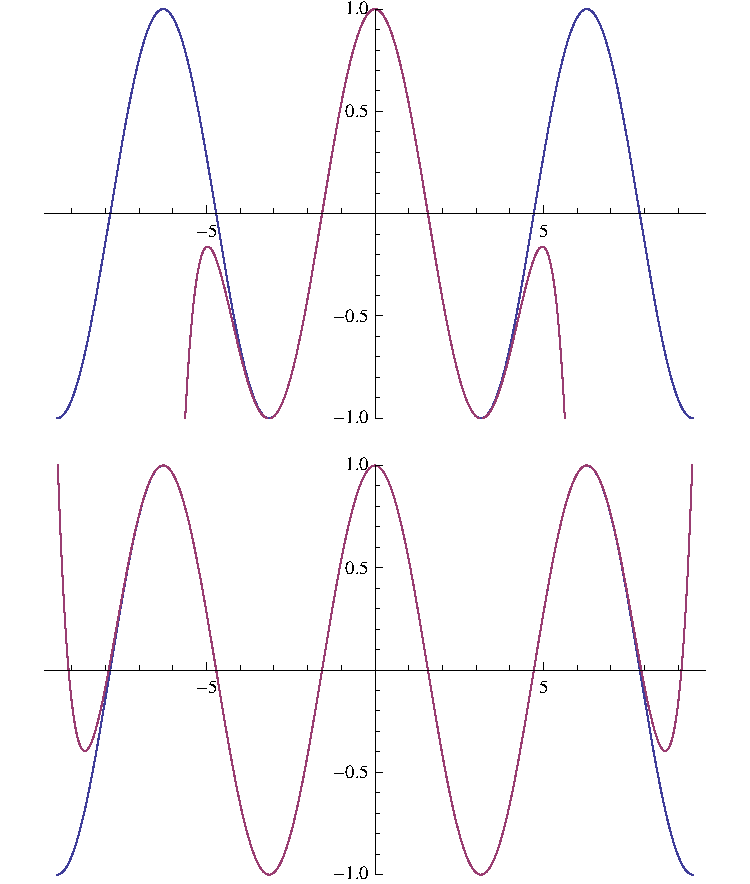
\includegraphics[width=\columnwidth]{../figures/taylor}
\caption{Truncated Taylor expansion with 11 terms (top) and 21 terms (bottom)}
\end{figure}
\end{columns}

\end{frame}

%------------------------------------------------

\begin{frame}
\frametitle{Shortcomings of the Taylor series expansion}
\begin{itemize}
	\item Numerical evaluation of high order derivatives is \alert{very noise
		sensitive and infeasible.}
	\item Truncations of the Whittaker-Shannon interpolation of all 
		$f \in \mathbf{BL}(\pi)$ has the following properties
		\begin{itemize}
			\item belongs to $f \in \mathbf{BL}(\pi)$
			\item converges uniformly in $L^2$
			\item if $A$ is a filter, then
				\begin{equation*}
					A[f](t) = \sum_{n=-\infty}^{\infty} f(n) A[\mathrm{sinc}](t-n)
				\end{equation*}
		\end{itemize}
		In stark contrast, \alert{none of these important properties hold} for
		truncations of a Taylor series expansion of any $f \in \mathbf{BL}(\pi)$.
		% TODO: Obliterates spectrum (?)
\end{itemize}
\end{frame}

%------------------------------------------------

\begin{frame}
\frametitle{Comparison: Taylor/Fourier series}
\begin{table}
\begin{tabular}{c c c}
\toprule
Expansion & \textbf{Fourier} & \textbf{Taylor}\\
\midrule
Physical Interpret. & Frequency component & Gradient component \\
Approx. & Global & \textcolor{blue}{Local} \\
Basis			& $e^{i \frac{\pi n}{T} t}$ & $\frac{(t-t_0)^n}{n!}$ \\
Basis type 		 & Sinusoids & Monomials \\
Basis Orthog.& \textcolor{blue}{Yes} & \alert{No} \\
Coefficient & $\frac{1}{2L} \int_{-L}^{L} f(t) e^{-i \frac{\pi n}{L} t} dt$ & $\mathcal{D}^n[f](t_0)$ \\
Coef. type  & Integral & \alert{Derivative} \\
\bottomrule
\end{tabular}
\end{table}

\begin{itemize}
	\item Can we find a better base for the space of linear differential operators?
	\item Furthermore, an \alert{orthogonal basis}?
\end{itemize}
\end{frame}

%------------------------------------------------
\section{Background}
%------------------------------------------------

\subsection{Chromatic Derivatives}

\begin{frame}
\frametitle{Overview of Chromatic Derivatives}
\begin{itemize}
	\item Dr. Aleks Ignjatovic introduced the concept of \textit{Chromatic Derivatives} 
	(c.f. \cite{Ignjatovic2009} for recent publication)
	\item \textbf{Key Concept:} Instead of $n$th-order derivatives, consider linear 
	combinations of lower order derivatives
	\begin{equation}
		\mathcal{D}_t^n \leftarrow P_n(\mathcal{D}_t) = \sum_{k=0}^{n} c_k \mathcal{D}_t^k
	\end{equation}
	where $P_n$ is an \alert{orthogonal polynomial}. E.g.
	\begin{itemize}
		\item Legendre polynomyials
		\item Chebyshev polynomials
		\item Hermite polynomials
		\item Et cetera.
	\end{itemize}
\end{itemize}
\end{frame}

%------------------------------------------------

\begin{frame}
\frametitle{Chromatic Derivatives}
\framesubtitle{Associated with Legendre Polynomials}
\begin{itemize}
\item Solutions to Legendre's differential equation
\begin{equation*}
\frac{d}{dx}\left[(1-x^2)\frac{d}{dx}P_n(x)\right]+n(n+1)P_n(x)=0
\end{equation*}
\item Defined by the recurrence
\begin{align*}
P_0(x) &= 1, P_1(x) = x \\
P_{n+1}(x) &= \frac{2n+1}{n+1}xP_n(x) - \frac{n}{n+1}P_{n-1}(x)
\end{align*}
\item \alert{Orthogonal} and \alert{complete} over $[-1, 1]$
\begin{equation*}
\int_{-1}^{1} P_n(x)P_m(x) dx = \frac{2}{2n+1} \delta_{mn}
\end{equation*}
where $\delta_{mn}$ is the Kronecker delta.
\end{itemize}
\end{frame}

%------------------------------------------------


\begin{frame}
\frametitle{Chromatic Derivatives}
\framesubtitle{Associated with Legendre Polynomials}
\begin{columns}[c]
\column{.55\textwidth}
\begin{itemize}
	\item Rescale and normalize
		over $[-\pi, \pi]$
	\begin{equation*}
		P_n^L(x) = \sqrt{2n+1}P_n\left(\frac{x}{\pi}\right)
	\end{equation*}
	\item \alert{Orthogonal} and \alert{complete} over $[-\pi, \pi]$
	\begin{equation*}
		\frac{1}{2\pi} \int_{-\pi}^{\pi} P_n^L(x) P_m^L(x) dx = \delta_{mn}
	\end{equation*}
\end{itemize}
\column{.35\textwidth}
\begin{figure} %[!ht]
\centering
	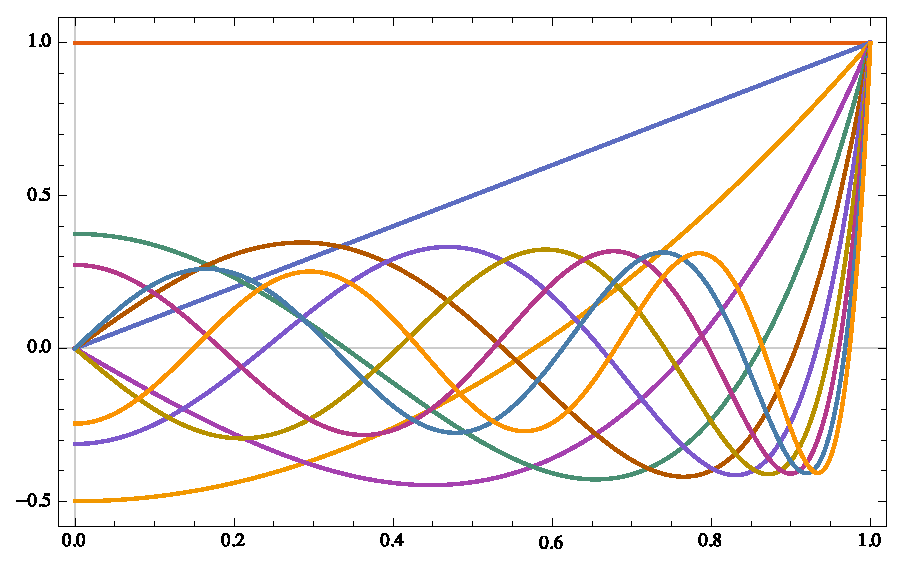
\includegraphics[width=\columnwidth]{../figures/legendre}
\caption{First 10 Legendre polynomials}
\end{figure}
\end{columns}
\begin{example}[First few Legendre polynomials]
\begin{align*}
& P_0(x) = 1, & P_2(x) = \frac{1}{2}(3x^2-1), \\
& P_1(x) = x, 
& P_3(x) = \frac{1}{2}(5x^3-3x)
\end{align*}
\end{example}
\end{frame}

%------------------------------------------------

\begin{frame}
\frametitle{Chromatic Derivatives}
The chromatic derivatives associated with Legendre polynomials of order $n$ 
with respect to $t$ is defined as
\begin{equation}
	\mathcal{K}_t^n = (-i)^n P_n^L(i\mathcal{D}_t)
\end{equation}
where $\mathcal{D}_t$ is the differential operator with respect to $t$ and
$P_n^L$ are the normalized and scaled Legendre polynomials.
\begin{example}[Derivative vs. chromatic derivative]
\begin{table}
\begin{tabular}{l l}
 & Operator \\
\midrule
Derivative & $\mathcal{D}_t^3$ \\
Chromatic Derivative & $\mathcal{K}_t^3 = \frac{\sqrt{7}}{2\pi} \left ( \frac{5}{\pi^2} \mathcal{D}_t^3 + 3 \mathcal{D}_t \right )$ \\
\bottomrule
\end{tabular}
\caption{A 3rd order derivative and 3rd order chromatic derivative}
\end{table}
\end{example}
\end{frame}

%------------------------------------------------

\begin{frame}
\frametitle{Chromatic Derivatives}
\begin{itemize}
	\item We can easily verify that
		\begin{equation*}
			\mathcal{K}_t^n[e^{i\omega t}] = i^n P_n^L(\omega) e^{i\omega t}
		\end{equation*}
	\item So for $f \in \mathbf{BL}(\pi)$, we have
		\begin{equation*}
			\mathcal{K}^n[f](t) = \frac{1}{2\pi} \int_{-\pi}^{\pi} i^n P_n^L(\omega) \hat{f}(\omega) e^{i\omega t} d\omega
		\end{equation*}
		by the inverse Fourier transform.
\end{itemize}
\end{frame}

%------------------------------------------------

\begin{frame}
\frametitle{Chromatic Derivatives}
\begin{itemize}
	\item The Fourier series expansion of $\hat{f}(\omega)$ is given by
		 \begin{align*}
			\hat{f}(\omega)	&= \sum_{n=0}^{\infty} c_n (-i)^n P_n^L(\omega) \\
			c_n							&= \frac{1}{2\pi} \int_{-\pi}^{\pi} i^n P_n^L(\omega) \hat{f}(\omega) d\omega
										= \mathcal{K}^n[f](0)
		\end{align*}
	\item By taking the inverse Fourier transform on $\omega$, we get
		\begin{align*}
			f(t)	&= \sum_{n=0}^{\infty} c_n (-1)^n \mathcal{K}^n[\mathrm{sinc}](t)
					= \sum_{n=0}^{\infty} c_n \sqrt{2n+1} j_n(\pi t)\\
			c_n		&= \mathcal{K}^n[f](0)
		\end{align*}
		where $j_n(t) = \sqrt{\frac{\pi}{2x}}J_{n+1/2}(x)$ is the spherical Bessel function of the first kind.
\end{itemize}
\end{frame}

% %------------------------------------------------

% \begin{frame}
% \frametitle{Table}
% \begin{table}
% \begin{tabular}{l p{2cm} p{2cm} p{2cm}}
% \toprule
% & \textbf{Taylor expansion} & \textbf{Chromatic expansion} & \textbf{Shannon-Whittaker expansion}\\
% \midrule
% Treatment 1 & 0.0003262 & 0.562 & \\
% Treatment 2 & 0.0015681 & 0.910 & \\
% Treatment 3 & 0.0009271 & 0.296 & \\
% \bottomrule
% \end{tabular}
% \caption{Table caption}
% \end{table}
% \end{frame}

%------------------------------------------------

\subsection{Related work}

\begin{frame}
\frametitle{Blocks of Highlighted Text}
\begin{block}{Block 1}
Lorem ipsum dolor sit amet, consectetur adipiscing elit. Integer lectus nisl, ultricies in feugiat rutrum, porttitor sit amet augue. Aliquam ut tortor mauris. Sed volutpat ante purus, quis accumsan dolor.
\end{block}

\begin{block}{Block 2}
Pellentesque sed tellus purus. Class aptent taciti sociosqu ad litora torquent per conubia nostra, per inceptos himenaeos. Vestibulum quis magna at risus dictum tempor eu vitae velit.
\end{block}

\begin{block}{Block 3}
Suspendisse tincidunt sagittis gravida. Curabitur condimentum, enim sed venenatis rutrum, ipsum neque consectetur orci, sed blandit justo nisi ac lacus.
\end{block}
\end{frame}

%------------------------------------------------

\begin{frame}
\frametitle{Multiple Columns}
\begin{columns}[c] % The "c" option specifies centered vertical alignment while the "t" option is used for top vertical alignment

\column{.45\textwidth} % Left column and width
\textbf{Heading}
\begin{enumerate}
\item Statement
\item Explanation
\item Example
\end{enumerate}

\column{.5\textwidth} % Right column and width
Lorem ipsum dolor sit amet, consectetur adipiscing elit. Integer lectus nisl, ultricies in feugiat rutrum, porttitor sit amet augue. Aliquam ut tortor mauris. Sed volutpat ante purus, quis accumsan dolor.

\end{columns}
\end{frame}

\begin{frame}
\frametitle{Table}
\begin{table}
\begin{tabular}{l l l}
\toprule
\textbf{Treatments} & \textbf{Response 1} & \textbf{Response 2}\\
\midrule
Treatment 1 & 0.0003262 & 0.562 \\
Treatment 2 & 0.0015681 & 0.910 \\
Treatment 3 & 0.0009271 & 0.296 \\
\bottomrule
\end{tabular}
\caption{Table caption}
\end{table}
\end{frame}

%------------------------------------------------

\begin{frame}
\frametitle{Theorem}
\begin{theorem}[Mass--energy equivalence]
$E = mc^2$
\end{theorem}
\end{frame}


\begin{frame}
\frametitle{Plot}
\begin{figure} %[!ht]
\centering
	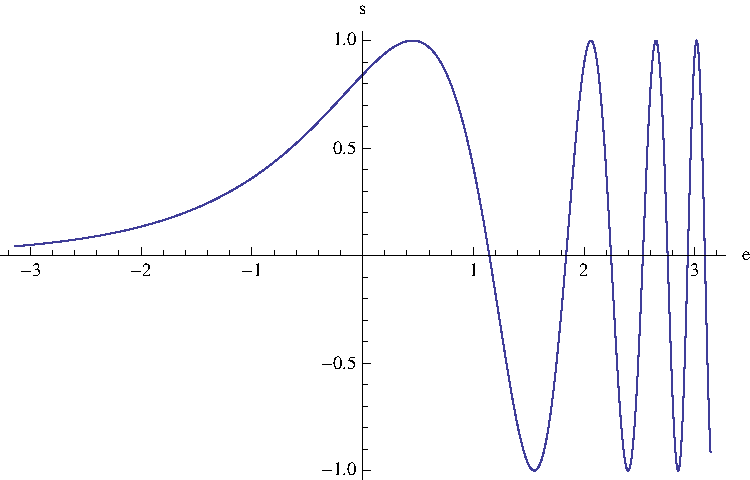
\includegraphics[width=0.8\columnwidth]{../figures/sin_exp_plot.pdf}
\end{figure}
\end{frame}


%------------------------------------------------

\begin{frame}[fragile] % Need to use the fragile option when verbatim is used in the slide
\frametitle{Verbatim}
\begin{example}[Theorem Slide Code]
\begin{verbatim}
\begin{frame}
\frametitle{Theorem}
\begin{theorem}[Mass--energy equivalence]
$E = mc^2$
\end{theorem}
\end{frame}\end{verbatim}
\end{example}
\end{frame}

%------------------------------------------------

\section{Proposal}

\begin{frame}
\frametitle{Figure}
Uncomment the code on this slide to include your own image from the same directory as the template .TeX file.
%\begin{figure}
%\includegraphics[width=0.8\linewidth]{test}
%\end{figure}
\end{frame}

%------------------------------------------------

\begin{frame}[fragile] % Need to use the fragile option when verbatim is used in the slide
\frametitle{Citation}
An example of the \verb|\cite| command to cite within the presentation:\\~

This statement requires citation \cite{Ignjatovic2009}.
\end{frame}

%------------------------------------------------

\section{Summary}

\subsection{Bibliography}

\begin{frame}[allowframebreaks]
Portions of this talk are derived from previous talks given by \cite{Ignjatovic2011,Liu2011}.
\end{frame}

\begin{frame}[allowframebreaks]
	\frametitle{References}
	\bibliographystyle{plain}
	\bibliography{../bibliography}
\end{frame}

%------------------------------------------------

\begin{frame}
\Huge{\centerline{The End}}
\end{frame}

%----------------------------------------------------------------------------------------

\end{document} 